\documentclass{beamer}

% Beamer style
%\usetheme[secheader]{Madrid}
\usetheme{CambridgeUS}
\usecolortheme[rgb={0.65,0.15,0.25}]{structure}
%\usefonttheme[onlymath]{serif}
\beamertemplatenavigationsymbolsempty
%\AtBeginSubsection

% Packages
%\usepackage[french]{babel}
\usepackage[latin1]{inputenc}
\usepackage{color}
\usepackage{dsfont, stmaryrd}
\usepackage{amsmath, amsfonts, amssymb}
\usepackage{stmaryrd}
\usepackage{epsfig}
\usepackage{array}
\usepackage{url}
\usepackage{/media/donnees/LATEX/astats}
%\usepackage[all]{xy}
\usepackage{graphicx}

% Commands
\definecolor{darkred}{rgb}{0.65,0.15,0.25}
\newcommand{\emphase}[1]{\textcolor{darkred}{#1}}
\newcommand{\ppause}{}
%\newcommand{\emphase}[1]{{#1}}
\newcommand{\paragraph}[1]{\textcolor{darkred}{#1}}
\newcommand{\refer}[1]{\textcolor{blue}{[\cite{#1}]}}
\newcommand{\Refer}[1]{\textcolor{blue}{[#1]}}
\newcommand{\newblock}{}

% Symbols
\newcommand{\Abf}{{\bf A}}
\newcommand{\Bias}{\mathbb{B}}
\newcommand{\Bbf}{{\bf B}}
\newcommand{\Beta}{\text{B}}
\newcommand{\Bcal}{\mathcal{B}}
\newcommand{\BIC}{\text{BIC}}
\newcommand{\Cbf}{{\bf C}}
\newcommand{\dd}{\text{d}}
\newcommand{\dbf}{{\bf d}}
\newcommand{\Dcal}{\mathcal{D}}
\newcommand{\Esp}{\mathbb{E}}
\newcommand{\Ebf}{{\bf E}}
\newcommand{\Ecal}{\mathcal{E}}
\newcommand{\Fbf}{{\bf F}}
\newcommand{\Gcal}{\mathcal{G}}
\newcommand{\Gbf}{{\bf G}}
\newcommand{\Gam}{\mathcal{G}\mbox{am}}
\newcommand{\Ibb}{\mathbb{I}}
\newcommand{\Ibf}{{\bf I}}
\newcommand{\ICL}{\text{ICL}}
\newcommand{\Jbf}{{\bf J}}
\newcommand{\Cov}{\mathbb{C}\text{ov}}
\newcommand{\Corr}{\mathbb{C}\text{orr}}
\newcommand{\Var}{\mathbb{V}}
\newcommand{\Vsf}{\mathsf{V}}
\newcommand{\pen}{\text{pen}}
\newcommand{\Fcal}{\mathcal{F}}
\newcommand{\Hbf}{{\bf H}}
\newcommand{\Hcal}{\mathcal{H}}
\newcommand{\Jcal}{\mathcal{J}}
\newcommand{\Kbf}{{\bf K}}
\newcommand{\Lbf}{{\bf L}}
\newcommand{\Lcal}{\mathcal{L}}
\newcommand{\Mcal}{\mathcal{M}}
\newcommand{\mbf}{{\bf m}}
\newcommand{\mum}{\mu(\mbf)}
\newcommand{\Ncal}{\mathcal{N}}
\newcommand{\Nbf}{{\bf N}}
\newcommand{\Nm}{N(\mbf)}
\newcommand{\Ocal}{\mathcal{O}}
\newcommand{\Obf}{{\bf 0}}
\newcommand{\Omegas}{\underset{s}{\Omega}}
\newcommand{\Pbf}{{\bf P}}
\newcommand{\Pcal}{\mathcal{P}}
\newcommand{\Qcal}{\mathcal{Q}}
\newcommand{\Rbb}{\mathbb{R}}
\newcommand{\Rbf}{{\bf R}}
\newcommand{\Rcal}{\mathcal{R}}
\newcommand{\sbf}{{\bf s}}
\newcommand{\Sbf}{{\bf S}}
\newcommand{\Scal}{\mathcal{S}}
\newcommand{\Ucal}{\mathcal{U}}
\newcommand{\Vcal}{\mathcal{V}}
\newcommand{\Tbf}{{\bf T}}
\newcommand{\ubf}{{\bf u}}
\newcommand{\Ubf}{{\bf U}}
\newcommand{\Vbf}{{\bf V}}
\newcommand{\Wbf}{{\bf W}}
\newcommand{\xbf}{{\bf x}}
\newcommand{\Xbf}{{\bf X}}
\newcommand{\ybf}{{\bf y}}
\newcommand{\Ybf}{{\bf Y}}
\newcommand{\zbf}{{\bf z}}
\newcommand{\Zbf}{{\bf Z}}
\newcommand{\betabf}{\mbox{\mathversion{bold}{$\beta$}}}
\newcommand{\pibf}{\mbox{\mathversion{bold}{$\pi$}}}
\newcommand{\Sigmabf}{\mbox{\mathversion{bold}{$\Sigma$}}}
\newcommand{\gammabf}{\mbox{\mathversion{bold}{$\gamma$}}}
\newcommand{\mubf}{\mbox{\mathversion{bold}{$\mu$}}}
\newcommand{\nubf}{\mbox{\mathversion{bold}{$\nu$}}}
\newcommand{\Thetabf}{\mbox{\mathversion{bold}{$\Theta$}}}
\newcommand{\thetabf}{\mbox{\mathversion{bold}{$\theta$}}}
\newcommand{\BP}{\text{BP}}
\newcommand{\EM}{\text{EM}}
\newcommand{\VEM}{\text{VEM}}
\newcommand{\VBEM}{\text{VB}}
\newcommand{\cst}{\text{cst}}
\newcommand{\obs}{\text{obs}}
\newcommand{\ra}{\emphase{\mathversion{bold}{$\rightarrow$}~}}
\newcommand{\QZ}{Q_{\Zbf}}
\newcommand{\Qt}{Q_{\thetabf}}

%====================================================================
\title[Statistical tools for segmentation]{Some statistical tools for change-points detection}

\author[Robin]{S. Robin, joint work with E. Lebarbier \& F. Picard}

\institute[AgroParisTech / INRA]{AgroParisTech / INRA \\
  \bigskip
  \begin{tabular}{ccccc}
    % 
\epsfig{file=../Figures/LogoINRA-Couleur.ps, width=2.5cm} & 
    % \hspace{.5cm} &
    % 
\epsfig{file=../Figures/logagroptechsolo.eps, width=3.75cm} & 
    % \hspace{.5cm} &
    % 
\epsfig{file=../Figures/logo-ssb.eps, width=2.5cm} \\ 
    
\epsfig{file=../Figures/LogoINRA-Couleur.ps, width=1.5cm} & 
    \hspace{.5cm} &
    
\epsfig{file=../Figures/logagroptechsolo.eps, width=2.25cm} & 
    \hspace{.5cm} &
    
\epsfig{file=../Figures/logo-ssb.eps, width=1.5cm} \\ 
  \end{tabular} \\
  \bigskip
  }

\date[COST ES-0601]{Homogenization in Climatological Databases,
  Octobre 2011, Budapest} 
%====================================================================

%====================================================================
%====================================================================
\begin{document}
%====================================================================
%====================================================================
\frame{\titlepage}

%====================================================================
%====================================================================
\section {Introduction}
%====================================================================
\frame{\frametitle{Introduction} \pause

  \begin{tabular}{cc}
    \hspace{-.5cm}
    \begin{tabular}{p{.5\textwidth}}
      Segmentation problems arise in many fields. \\
      \\
      \paragraph{General aim:} %\\
      Given a series of observations, find abrupt change-points in their
      distribution.
    \end{tabular}
    & 
    \hspace{-.5cm}
    \begin{tabular}{p{.5\textwidth}}
      \epsfig{file=../Figures/bt474_c1_seg_homo_K10.eps, clip=,
      width=.4\textwidth} 
    \end{tabular}
  \end{tabular}

%  \item Within multiple series of measurements,
%  \item In presence of correlation between the series.

  \pause\bigskip
%   \begin{tabular}{lccc}
  \begin{tabular}{p{.2\textwidth}ccc}
    \emphase{Examples:} & \emphase{Genomics} &
    \emphase{Meteorology} & \emphase{Geography} \pause \\
%    \hline    
%    \emphase{Series $m$} & Patients & Station & Station \\
    \hline    
    \emphase{'Time' $t$} & Position along & Time & Time  \\
    & the genome &  &  \pause\\
    \hline    
    \emphase{Signal $Y_{tm}$} & Micro-array & Temperature & GPS
    location \pause \\ 
    \hline    
    \emphase{Breakpoints} & Endpoints of & Change of &
    Earth's crust \\ 
    \emphase{$\{\tau_k\}$} & altered regions & instrument & shifts \\
 %   \hline    
 %   \emphase{Correlation $\Sigmabf$} & Probe effect & Spatial & Spatial \\
  \end{tabular}
}

%====================================================================
\frame{\frametitle{Issues} 
  
  Segmentation raises both statistical and algorithmic issues. \pause \\
  ~\\

  \paragraph{Statistics:}
  \begin{itemize}
  \item definition of the statistical model;
  \item inference of the change-point location;
  \item choice of the number of segments.
  \end{itemize}
  \pause
  
  \paragraph{Algorithmics:}
  \begin{itemize}
  \item optimal repartition of the change-points,
  \item efficient exploration of the segmentation space.
  \end{itemize}
  \pause
  
  \paragraph{Outline.}
  \begin{enumerate}
  \item Segmentation of one single series;
  \item Joint segmentation of several series;
  \item CGHseg package.
  \end{enumerate}
  }

%====================================================================
%====================================================================
\section{One series}
\subsection {Statistical model}
%====================================================================
\frame{\frametitle{One Series} \pause
  
  \begin{tabular}{cc}
    \hspace{-.5cm}
    \begin{tabular}{p{.5\textwidth}}
      \onslide+<2->{\paragraph{Statistical model.} 
        \begin{itemize}
        \item $\text{Signal} = f(\text{Time})$; \\}
        \onslide+<3->{
        \item Change-points positions: \\
          $\tau_1, \tau_2, ..., \tau_{K-1};$ \\}
        \onslide+<4->{
        \item Means signal level within each interval: \\
          $\mu_1, \mu_2, ..., \mu_K$; \\}
        \onslide+<5->{
        \item Observed signal at time $t=$ \\
          mean + noise $\Ncal(0, \sigma�)$.
        \end{itemize}}
    \end{tabular}
    & 
    \hspace{-1cm}
    \begin{tabular}{c}
      \begin{overprint}
        \onslide<2>
        $\qquad \qquad \;\;\, Y_t =$ \\
        \epsfig{file=../Figures/FigSeg-Budapest-1.eps, clip=,
          angle=270, width=.5\textwidth} 
        \onslide<3>
        if $t \in \textcolor{blue}{I_k}, \quad Y_t =$ \\
        \epsfig{file=../Figures/FigSeg-Budapest-2.eps, clip=,
          angle=270, width=.5\textwidth} 
        \onslide<4>
        if $t \in \textcolor{blue}{I_k}, \quad Y_t = \textcolor{red}{\mu_k}$ \\
        \epsfig{file=../Figures/FigSeg-Budapest-3.eps, clip=,
          angle=270, width=.5\textwidth} 
        \onslide<5->
        if $t \in \textcolor{blue}{I_k}, \quad Y_t =
        \textcolor{red}{\mu_k} + E_t$ \\ 
        \epsfig{file=../Figures/FigSeg-Budapest-4.eps, clip=,
          angle=270, width=.5\textwidth} 
      \end{overprint}
    \end{tabular}
  \end{tabular}

  \onslide+<6->{
    \paragraph{Aim:}
    Retrieve the 'true' number of segments \emphase{$K$},
    change-points locations \emphase{$(\tau_k)$} and means
    \emphase{$(\mu_k)$} ... within a reasonable time \refer{Lav05}.
  }

}

%====================================================================
\subsection {Algorithmics}
%====================================================================
\frame{\frametitle{Algorithmics} 

  \paragraph{Naive search.} There are ${{n-1}\choose{K-1}}$ possible
  ways to divide a series with length $n$ into $K$ segments ($n =
  1000$, $K = 10 \rightarrow 10^{21}$ possibilities). \\
  \centerline{
    \ra A naive search is \emphase{hopeless}. 
    }

  \bigskip\bigskip\pause
  Finding the optimal
  location of the change-points can be rephrased as a
  \emphase{shortest path problem}. 

  \bigskip\pause
  \paragraph{Dynamic programming (DP).}  allows to recover the
  \emphase{optimal segmentation} with $\Ocal(Kn^2)$ complexity,
  provided that the contrast to be optimized is \emphase{additive}:
  %e.g.
  %$$
  %\log p (\Ybf) = \sum_k \log p (\Ybf^k)
  %$$
  \centerline{
    \ra Observations from different segments are \emphase{considered as 
      independent}. }

  \bigskip\bigskip\pause
  \paragraph{'Pruned' dynamic programming (PDP).}  For 'nice'
  contrasts (e.g. least squares), the optimal segmentation can be
  retrieved in $OK (n \log n)$ \refer{Rig10}.

}

%====================================================================
\subsection {Model selection}
%====================================================================
\frame{\frametitle{Model selection: $K = ?$} 

  \paragraph{How many segments?}
  The fit of the segmentation improves as $K$ increases.

  \bigskip \pause
  \begin{tabular}{cc}
    \hspace{-.51cm}
    \begin{tabular}{p{.55\textwidth}}
      \emphase{Numerous criteria} have been proposed
      \begin{itemize}
      \item Penalized likelihood \refer{Lav05,Leb05};
      \item BIC \refer{ZhS07};
      \item ICL \refer{RLR11};
      \item ...
      \end{itemize}
    \end{tabular}
    & 
    \hspace{-1cm}
    \begin{tabular}{p{.5\textwidth}}
      \epsfig{file = ../Figures/Select_K.ps, clip=, bbllx=146, bblly=529,
        bburx=464, bbury=777, width=.4\textwidth} 
    \end{tabular}
  \end{tabular}

  \medskip \pause
  \paragraph{In practice: } 
  \begin{itemize}
  \item This turns out to be the \emphase{most delicate
    problem}...
  \item \emphase{Do we always need to know} the number of segments?
  \end{itemize}
}

%====================================================================
\subsection {Breakpoint location}
%====================================================================
\frame{\frametitle{Breakpoint location} 

  \begin{tabular}{cc}
    \hspace{-.5cm}
    \begin{tabular}{p{.5\textwidth}}
      \onslide+<1->{
        \paragraph{Discrete nature of change-points $(\tau_k)$} \ra standard
        inference does not apply. \\ \\
      }
      \onslide+<2->{
        \paragraph{The posterior} distribution of the $(\tau_k)$
        can be computed, via the exploration of the \emphase{whole
        segmentation space}.  \\ \\
      }
      \onslide+<3->{
        \paragraph{Complexity:} This can be done with the same
        complexity as dynamic programming: $O(Kn�)$. \\
        \refer{RLR11}.
      }
    \end{tabular}
    & 
    \hspace{-1cm}
    \begin{tabular}{p{.5\textwidth}}
      \onslide+<1->{
        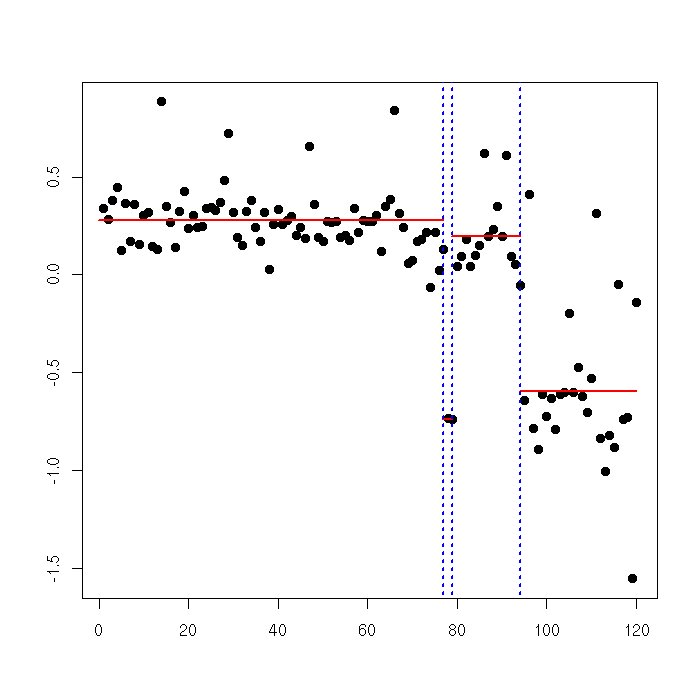
\includegraphics[width=0.5\textwidth, height=0.4\textheight,
        clip=]{../Figures/CopyNumberChr10_ICL}  \\ 
      }
      \onslide+<2->{
        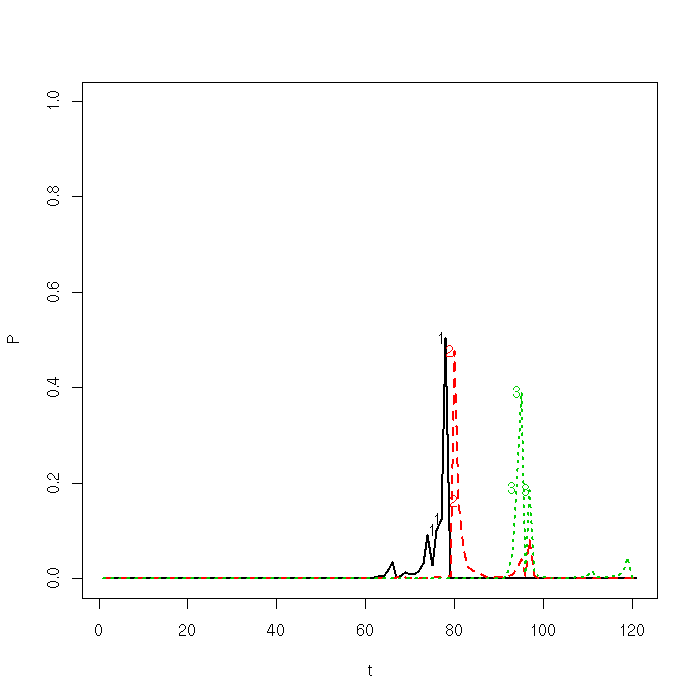
\includegraphics[width=0.5\textwidth, height=0.4\textheight,
        clip=]{../Figures/CopyNumberChr10_ProbaICL}  
      }
    \end{tabular}
  \end{tabular}
}

%====================================================================
%====================================================================
\section {Multiple series}
\subsection {Simultaneous vs joint segmentation}
%====================================================================
\frame{\frametitle{Multiple series} \pause

  \begin{tabular}{cc}
    \hspace{-.5cm}
    \begin{tabular}{p{.5\textwidth}}
      \onslide+<2->{
        One often deals with multiple series, observed 
        \begin{itemize}
        \item at \emphase{different locations} or
        \item for \emphase{different patients}.
        \end{itemize}
        }
      \bigskip
      \onslide+<3->{
        Series can be analyzed either \emphase{independently} or
        \emphase{jointly}. }  \\
        ~\\
        \onslide+<4->{
          Joint analysis allows to \emphase{share information} among
          the series to avoid \emphase{spurious change-point}
          detection. }
    \end{tabular}
    & 
    \hspace{-.5cm}
    \begin{tabular}{p{.5\textwidth}}
      \onslide+<4->{
        \epsfig{file= ../Figures/profils2_9_29.ps,
          width=.45\textwidth, height=.8\textheight, clip=} 
        }
    \end{tabular}
  \end{tabular}

  % \bigskip\bigskip\pause
  % \paragraph{2-stage dynamic programming.} A 2-stage algorithm can be
  % derived to recover the optimal segmentation of $M$
  % \emphase{independent series}, under the same assumption
  % \refer{PLH11}.  
}

%====================================================================
\subsection {Modelling the dependency}
%====================================================================
\frame{\frametitle{Accounting for dependency} 

  Information can be shared between series if they are
  \emphase{correlated}. 

  \centerline{
    \ra \emphase{This contradicts the 'independence'} assumption used
    in DP. 
    }

  \vspace{-1.5cm}
  \begin{tabular}{cc}
    \hspace{-.5cm}
    \begin{tabular}{p{.4\textwidth}}
      \onslide+<2->{\paragraph{One series:} OK with
        classical DP. \\}
      \onslide+<3->{\smallskip
        \paragraph{Independent series:}
        OK with 2-stage dynamic programming. \\}
      \onslide+<4->{\smallskip
        \paragraph{Simultaneous segmentation:} Same complexity as for
      one series \ra classical DP. \\} 
    \end{tabular}
    & 
    \hspace{-.5cm}
    \begin{tabular}{p{.5\textwidth}}
      \vspace{1.75cm}
      \begin{overprint}
        \onslide<2>
        \epsfig{file=../Figures/SegFA-ModGraph-X1.eps, clip=,
          width=0.7\textwidth}
        \onslide<3>
        \epsfig{file=../Figures/SegFA-ModGraph-X1m.eps, clip=,
          width=0.7\textwidth}
        \onslide<4>
        \epsfig{file=../Figures/SegFA-ModGraph-XcovSimult.eps, clip=,
          width=0.7\textwidth}
        \onslide<5->
        \epsfig{file=../Figures/SegFA-ModGraph-Xcov.eps, clip=,
          width=0.7\textwidth}
      \end{overprint}
    \end{tabular}
  \end{tabular}  

  \onslide+<5->{
    \vspace{-2cm}
    \paragraph{Joint segmentation:} Non-additivity
    of the contrast \ra \emphase{DP cannot apply as such}.} 

  }


%====================================================================
\subsection {Random effects and factor models}
%====================================================================
% \frame{ \frametitle{Modelling the dependency}
 
%   Correlation between series can be due to a \emphase{common (latent)
%     effect} affecting all of them.

%   \begin{tabular}{cc}
%     \hspace{-.5cm}
%     \begin{tabular}{p{.5\textwidth}}
%       \onslide+<2->{
%         \paragraph{Random effect:} Random (unobserved)
%         term $Z_t$ at each time. \\
%         ~\\}
%       \begin{tabular}{rll}
%         \onslide+<3->{
%           \paragraph{Model:} & 
%           Observed signal & $Y_{t, s}$ \\ ~\\
%           = & \textcolor{red}{segment mean} & $\mu_{k, s}$ \\ ~\\}
%         \onslide+<4->{
%           + & \textcolor{green}{random effect} & $Z_t$ \\ ~\\}
%         \onslide+<5->{
%           + & error term & $E_{t, s}$ \\
%           ~ 
%         }
%       \end{tabular}
%       \onslide+<6->{\refer{PLB11}}
%     \end{tabular}
%     & 
%     \hspace{-1cm}
%     \begin{tabular}{c}
%       \vspace{-1cm}
%       \begin{overprint}
%         \onslide<2>
%         \epsfig{file=../Figures/FigSegMult-Budapest-1.eps, clip=,
%           width=.5\textwidth, height=.8\textheight} 
%         \onslide<3>
%         \epsfig{file=../Figures/FigSegMult-Budapest-2.eps, clip=,
%           width=.5\textwidth, height=.8\textheight} 
%         \onslide<4>
%         \epsfig{file=../Figures/FigSegMult-Budapest-3.eps, clip=,
%           width=.5\textwidth, height=.8\textheight} 
%         \onslide<5->
%         \epsfig{file=../Figures/FigSegMult-Budapest-4.eps, clip=,
%           width=.5\textwidth, height=.8\textheight} 
%       \end{overprint}
%     \end{tabular}
%   \end{tabular}
% }
\frame{ \frametitle{Modelling the dependency}

  The dependence between the series at each time $t$ is described by the
  correlation matrix
  $$
  \Rbf = [\rho_{s, s'}]: \qquad \rho_{s, s'} = \Corr(Y_{t, s}, Y_{t,
    s'}).
  $$

  \pause
  \paragraph{Various correlation shapes.}
  \begin{itemize}
  \item \emphase{Uniform}: for all series $s$ and $s'$, $\rho_{s, s'}
    = \rho$ \refer{PLB11}.
  \item \emphase{Spatial}: depending on the distance between the stations where
    series were collected: $\rho_{s, s'} = e^{-d(s, s')}$.
  \item \emphase{Arbitrary form}: $\rho_{s, s'} = \rho_{s, s'}$.
  \end{itemize}

  \bigskip\pause
  \paragraph{Interesting rewriting.}
   For any correlation matrix $\Rbf$, one can define a matrix
   $\Bbf$ such that
   $$
   \Rbf = \Corr(\Bbf \Zbf)
   $$
   where the elements of $\Zbf$ are i.i.d. standard Gaussian.  
 }

%====================================================================
\frame{\frametitle{Factor models and E-M inference} 

  \paragraph{Factor model} refers to the rewriting of the correlation
  matrix $\Rbf$ as $\Corr(\Bbf \Zbf)$ (Cholevsky's decomposition).

  \bigskip\pause
  \paragraph{Incomplete data model.} The factor model is said
  incomplete, as we do note observe the 'factor' $\Zbf$.  Indeed, its
  statistical inference would be \emphase{much easier} if we would
  observe it.

  \bigskip\pause
  \paragraph{E-M algorithm.} Maximum likelihood inference incomplete
  data model can be achieved via the E-M algorithm \refer{DLR77},
  which alternates
  \begin{itemize}
  \item \pause \emphase{E-step:} retrieve the expected values
    $\widehat{\Zbf}$ of the unknown $\Zbf$;
  \item \pause \emphase{M-step:} given $\widehat{\Zbf}$, estimate
    \begin{itemize}
    \item the signal means $\mu_{k, s}$,
    \item the change-point locations $\tau_{k, s}$ (via 2-stage DP) 
    \item and the correlation structure $\Rbf$.
    \end{itemize}
  \end{itemize}
}

%====================================================================
\frame{ \frametitle{Breaking down the dependency}

  \vspace{-1cm}      
  \begin{tabular}{cc}
    \hspace{-.5cm}
    \begin{tabular}{p{.4\textwidth}}  The corelation between series

      \onslide+<1->{\paragraph{The correlation between series} prevents
        from using DP\\}
      \onslide+<2->{\medskip
        \paragraph{The factor model} accounts for this 
        dependency. \\} 
      \onslide+<3->{\medskip
        \paragraph{Conditional independence:} Given the factors, the
        series are again independent. \\}  
    \end{tabular}
    & 
    \hspace{-.5cm}
    \begin{tabular}{p{.5\textwidth}}
      \vspace{1cm}      
      \begin{overprint}
        \onslide<1>
        \epsfig{file=../Figures/SegFA-ModGraph-Xcov.eps, clip=,
          width=0.7\textwidth}
        \onslide<2>
        \epsfig{file=../Figures/SegFA-ModGraph-XZ.eps, clip=,
          width=0.7\textwidth}
        \onslide<3>
        \epsfig{file=../Figures/SegFA-ModGraph-XcondZ.eps, clip=,
          width=0.7\textwidth}
        \onslide<4>
        \epsfig{file=../Figures/SegFA-ModGraph-XcondZ.eps, clip=,
          width=0.7\textwidth}
      \end{overprint}
    \end{tabular}
  \end{tabular}
  
  \onslide+<4>{
    \vspace{-1.25cm}
    \paragraph{DP-EM algorithm:} Iteratively \emphase{estimate} the latent
    variables $\widehat{\Zbf}$ and perform the segmentation using DP.
  }
}

%====================================================================
%====================================================================
\section {'CGHseg' R Package}
%====================================================================
\frame{\frametitle{CGHseg R Package} \pause

  \paragraph{CGHseg} is an R package dedicated to the analysis of
  Comparative Genomic Hybridization \refer{PLH11}.
  
  \bigskip\pause
  \paragraph{Linear model framework:} 
 
  \medskip
  \begin{tabular}{p{.2\textwidth}p{.35\textwidth}p{.35\textwidth}}
%     \emphase{Task} & \emphase{Representation} & \emphase{Model} \\   
%     \hline
%     \\
    \emphase{Segmentation} & regression on unknown $\Tbf$: &
    $\displaystyle{\Ybf = \Tbf \mubf + \Ebf}$ \pause \\ 
    \\
    \emphase{Correlation} & {Factor model(\footnote{uniform
        correlation}): $\Zbf$}  & 
    $\displaystyle{\sl \Ybf = \Tbf \mubf + \Lbf \Zbf + \Ebf}$ \pause \\ 
    \\
    \emphase{Correction} & fixed covariates effect: $\betabf$ &
    $\displaystyle{\Ybf = \Tbf \mubf + \Xbf \betabf + \Ebf}$ \pause \\  
    \\
    \emphase{Calling} & crosstabulation table $\Cbf$: &
    $\displaystyle{\Ybf = \Tbf \Cbf \mbf + \Ebf}$ \pause \\
    \\
    \emphase{Combinations} 
    & fixed + random effects: &
    $\displaystyle{\Ybf = \Tbf \mubf + \Xbf \betabf + \Lbf \Zbf + \Ebf}$ \\
    & fixed effects + calling: &
    $\displaystyle{\Ybf = \Tbf \Cbf \mbf + \Xbf \betabf + \Ebf}$  \\
  \end{tabular}

}


%====================================================================
\frame{\frametitle{An example of combination}

  \begin{tabular}{ccc}
    \onslide+<1->{\textcolor{red}{Segmentation}
      % +\textcolor{green}{calling}
    }
    & 
    \onslide+<2->{+ \textcolor{blue}{fixed effects} }
    & 
    \onslide+<3->{$\Ybf = \textcolor{red}{\Tbf} 
      %\textcolor{green}{\Cbf} 
      \mbf + \textcolor{blue}{\Xbf} \betabf + \Ebf$  }
    \\
    % \epsfig{file = ../Figures/PLH11-V1-Fig1.eps, clip=, angle=270,
    %   bbllx=10, bblly=0, bburx=300, bbury=840, scale=0.4}        
    \onslide+<1->{\epsfig{file = ../Figures/PLH11-V1-Fig1.eps, clip=,
        angle=270, bbllx=33, bblly=34, bburx=282, bbury=272,
        scale=0.4}}   
    & 
    \onslide+<2->{\epsfig{file = ../Figures/PLH11-V1-Fig1.eps,
        clip=, angle=270, bbllx=33, bblly=302, bburx=282, bbury=540,
        scale=0.4}} 
    & 
    \onslide+<3->{\epsfig{file = ../Figures/PLH11-V1-Fig1.eps, clip=,
        angle=270, bbllx=33, bblly=571, bburx=282, bbury=810,
        scale=0.4}}         
  \end{tabular}

  \bigskip
  \onslide+<4->{
    \begin{itemize}
    \item \emphase{Correction:} functional versions (spline, wavelets)
      for the probe effect.
    \item \emphase{Presentation} at
      \url{www.agrocampus-ouest.fr/math/useR-2009/}
    \item \emphase{\tt cran.r-project.org/web/packages/cghseg/index.html}
    \end{itemize}
  }
  
}

%====================================================================
\frame{\frametitle{Some simulations}

  \vspace{-0.5cm}
  \begin{tabular}{cc}
    \hspace{-0.5cm}
    \begin{tabular}{p{.5\textwidth}}
      Correction and calling improve
      \begin{itemize}
      \item estimation of $K$, 
      \item breakpoint detection (FDR / FNR), 
      \item true signal recovery.
      \end{itemize}
      
      \bigskip
      \paragraph{Calling:} yes = --, no = - -

      \bigskip
      \paragraph{Correction:} \\
      $\blacksquare =$ no correction, \\
      \textcolor{red}{$\bullet = $ position  specific}, \\
      \textcolor{blue}{$\triangle =$ spline}, \\
      \textcolor{green}{$\diamond =$ wavelet}, \\
      \textcolor{orange}{$\circ =$ CBS} 
    \end{tabular}
    &
    \hspace{-1cm}
    \begin{tabular}{p{.5\textwidth}}
      \epsfig{file = ../Figures/PLH11-V1-Fig2.eps, clip=,
        width=.5\textwidth, height=0.85\textheight}        
    \end{tabular}
  \end{tabular}

  }

%====================================================================
\frame{ \frametitle{}
  \tiny{
    \bibliography{/media/donnees/Biblio/AST,/media/donnees/Biblio/ARC}
    \bibliographystyle{/media/donnees/LATEX/astats}
    }
  }

%====================================================================
%====================================================================
\section {Appendix}
%====================================================================
\subsection{Comparative study}
%====================================================================
\frame{ \frametitle{Comparative study}
    \paragraph{\refer{LJK05}.} On both synthetic and
    real data (GBM brain tumor data), the CGHseg performs among the
    best for one serie analysis.
    $$
    % \epsfig{file = ../Figures/LPJ05-Fig1.eps, clip=, scale=1.2}
    % \epsfig{file = ../Figures/LPJ05-Fig3.eps, clip=, scale=1.2}
    \epsfig{file = ../Figures/LPJ05-Fig4.eps, clip=, scale=.6}
    $$
  }

%====================================================================
\subsection{Factor model}
%====================================================================
\frame{ \frametitle{Factor model}

  \paragraph{Joint segmentation model.}
  $$
  Y_{tm} = \mu_{km} + F_{tm},   
  \qquad \forall t \in I_k^{\emphase{m}}
  \qquad \Fbf_t \text{ \emphase{i.i.d.} } \sim \Ncal_M(\Obf,
  \emphase{\Sigmabf}). 
  $$

  \bigskip\pause
  \paragraph{Factor model:} If $\Sigmabf$ can be written as
   $$
   \emphase{\Sigmabf = \Bbf \Bbf' + \sigma^2 \Ibf}, 
   \qquad \text{with } \Bbf = [b_{qm}]: M \times Q, 
   \qquad Q < M
   $$ \pause
   (always true for $Q = M-1$), then the model can be rewritten as
   $$
   Y_{tm} = \mu_{km} + \sum_{q=1}^Q Z_{tq} b_{qm} + E_{tm},   
   \qquad \forall t \in I_k^{m}
   $$
   where
   $
   \Zbf_t \text{ \emphase{i.i.d.} } \sim \Ncal_Q(\Obf, \emphase{\Ibf}), 
   \quad
   \Ebf_t \text{ \emphase{i.i.d.} } \sim \Ncal_M(\Obf,
   \emphase{\sigma^2 \Ibf}), 
   \quad
   (\{\Zbf_t\}, \{\Ebf_t\}) \text{ indep.}
   $

   \bigskip\bigskip
   The same trick is used in \refer{FKC09} in a different context.
  }

%====================================================================
\subsection{Simulation study}
%====================================================================
\frame{ \frametitle{Simulations: an example}
  \begin{tabular}{cc}
    \hspace{-.5cm}
    \begin{tabular}{p{.5\textwidth}}
      $M = 5$ stations, $n = 50$ times; \\
      $\mu_k^m \in \{-2, -1, 0, 1, 2\}$ %\\
      %$d(m, m') = $ distance from $m$ to $m'$; 
      \begin{eqnarray*}
        \Sigma(m, m') & = & (1-\lambda) \rho^{d(m, m')} \\
        & + & \lambda \sigma^2 \Ibb\{m = m'\}
      \end{eqnarray*}
      \\
      \onslide+<2->{
        \paragraph{Relative fit} as compared to $(K_0, Q_0)$: 
        $$
        \text{e.g.} \qquad \frac{RMSE(K, Q)}{RMSE(K_0,
          Q_0)} - 1 
        $$
      %\vspace{-.25cm}
        $$
        \begin{array}{lccc}
          \onslide+<3->{
            (\%) & (K_0, \widehat{Q}) & 
            (\widehat{K}, Q_0) & (\widehat{K}, \widehat{Q}) \\
            \hline
%         \emphase{\Tbf\mubf} & \emphase{-0.15} & -0.06  & 0.10 \\
%         \emphase{\Sigmabf} & 23.9 & \emphase{3.0} & 78.7 \\
            \emphase{\Tbf\mubf} & -16 & -8 & -17 \\
            }
          \onslide+<4->{
            \emphase{\Sigmabf} & -0.8 & -1.8 & -0.7
            }
        \end{array}
        $$
        }
    \end{tabular}
    & 
    \hspace{-.5cm}
    \begin{tabular}{p{.5\textwidth}}
      \onslide+<3->{
        \vspace{-2cm}
        \epsfig{file=../Figures/FaSegSimEx.n49.M5kmean3FitTmu.ps,
          clip=, angle=270, width=.48\textwidth}  \\
        $\qquad \quad K_0 = 17, \qquad \widehat{K} = 16$ \\ 
        }
      \onslide+<4->{
      \vspace{-.5cm}
      \epsfig{file=../Figures/FaSegSimEx.n49.M5kmean3FitSigma.ps,
        clip=, angle=270, width=.48\textwidth} \\
      \vspace{-.5cm}
      $\quad Q_0 = M-1 = 4, \qquad \widehat{Q} = 1$
      }
%       \begin{overprint}
%       \end{overprint}
    \end{tabular}
  \end{tabular}

  }

%====================================================================
\frame{ \frametitle{Estimation of $K$ and $Q$}

  \vspace{-.25cm}
  {2 conditions:} \textcolor{red}{$M=5, n=50$},
  \textcolor{green}{$M=10, n=100$}, $Q_0 = M-1$, increasing $\sigma^2$
  \\
  \pause
  \begin{tabular}{cc}
%     $\widehat{K}-K_0$ for $Q = \widehat{Q}$ &
%     $\widehat{K}-K_0$ for $Q = Q_0$ \\
    \epsfig{file=../Figures/FAsegSimJDS-EstimK-Qest.ps,
      clip=, angle=270, width=.45\textwidth} &
    \epsfig{file=../Figures/FAsegSimJDS-EstimK-Q0.ps,
      clip=, angle=270, width=.45\textwidth} 
  \end{tabular}\\
  \vspace{-.5cm} \pause
  \begin{tabular}{cc}
%     $\widehat{Q}-Q_0$ for $K = \widehat{K}$ &
%     $\widehat{Q}-Q_0$ for $K = K_0$ \\
    \epsfig{file=../Figures/FAsegSimJDS-EstimQ-Kest.ps,
      clip=, angle=270, width=.45\textwidth} &
    \epsfig{file=../Figures/FAsegSimJDS-EstimQ-K0.ps,
      clip=, angle=270, width=.45\textwidth} 
  \end{tabular}
  }

%====================================================================
\frame{ \frametitle{Fit of the segmentation $\Tbf\mubf$}

  \begin{tabular}{cc}
    \hspace{-.5cm}
    \begin{tabular}{p{.6\textwidth}}
      \paragraph{Fit of the segmentation.} Measured in terms of RMSE:
      $$
      RMSE = \|\widehat{\Tbf\mubf} - \Tbf\mubf \|
      $$
      relatively to the reference case: $(K_0, Q_0)$. \\
      \\
      \onslide+<2->{
        \paragraph{Results} are overall quite good:
        \begin{itemize}
        \item Results are competitive when using $(\widehat{K},
          \widehat{Q})$;          
          \onslide+<3->{
          \item Using the true $Q_0$ does not improve much;
            }
          \onslide+<4->{
          \item Using the right number of segments $K_0$ does improve the
            fit.
            }
        \end{itemize}
        }
    \end{tabular}
    & 
    \hspace{-.5cm}
    \begin{tabular}{p{.3\textwidth}}
      \vspace{-1.5cm}
        \onslide+<2->{
          \epsfig{file=../Figures/FAsegSimJDS-EstimTmu-KeQe.ps,
            clip=, angle=270, width=.37\textwidth} \\
          }
        \onslide+<3->{
          \vspace{-.75cm}
          \epsfig{file=../Figures/FAsegSimJDS-EstimTmu-KeQo.ps,
            clip=, angle=270, width=.37\textwidth} \\
          }
        \onslide+<4->{
          \vspace{-.75cm}
          \epsfig{file=../Figures/FAsegSimJDS-EstimTmu-KoQe.ps,
            clip=, angle=270, width=.37\textwidth} 
          }
%       \begin{overprint}
%       \end{overprint}
    \end{tabular}
  \end{tabular}
  }

%====================================================================
\frame{ \frametitle{Fit of the variance structure $\Sigmabf$}

  \begin{tabular}{cc}
    \hspace{-.5cm}
    \begin{tabular}{p{.6\textwidth}}
      \paragraph{Fit of the variance.} Also measured in terms of RMSE
      relatively to the reference case: $(K_0, Q_0)$. \\
      \\
      \onslide+<2->{
        \paragraph{Results} are overall not that good:
        \begin{itemize}
        \item Results are bad when using $(\widehat{K},
          \widehat{Q})$;          
          \onslide+<3->{
          \item Using the \emphase{true $Q_0$ does not improve much
              (...!)}; 
            }
          \onslide+<4->{
          \item Using the right number of segments $K_0$ really does
            improve the fit.
            }
        \end{itemize}
        }
    \end{tabular}
    & 
    \hspace{-.5cm}
    \begin{tabular}{p{.3\textwidth}}
      \vspace{-1.5cm}
        \onslide+<2->{
          \epsfig{file=../Figures/FAsegSimJDS-EstimSigma-KeQe.ps,
            clip=, angle=270, width=.37\textwidth} \\
          }
        \onslide+<3->{
          \vspace{-.75cm}
          \epsfig{file=../Figures/FAsegSimJDS-EstimSigma-KeQo.ps,
            clip=, angle=270, width=.37\textwidth} \\
          }
        \onslide+<4->{
          \vspace{-.75cm}
          \epsfig{file=../Figures/FAsegSimJDS-EstimSigma-KoQe.ps,
            clip=, angle=270, width=.37\textwidth} 
          }
%       \begin{overprint}
%       \end{overprint}
    \end{tabular}
  \end{tabular}
  }


%====================================================================
%====================================================================
\end{document}
%====================================================================
%====================================================================

